\chapter{Object Recognition}
\label{cha:objrecog}

\begin{chapterabstract}
In this chapter, we address the problem of object class recognition. To approach this challenge, we rely on the geometric information provided by 3D object representations such as point clouds. Furthermore, we focus on learning-based methods to distinguish objects from different classes while capturing the variability of shape of different objects which belong to the same class. More specifically, we leverage deep learning for such task. The chapter begins introducing and formulating the object recognition task in Section \ref{cha:objrecog:sec:introduction} followed by a review of the most relevant literature and datasets in Sections \ref{cha:objrecog:sec:relatedworks} and \ref{cha:objrecog:sec:datasets}. After that, we present our first proposal for 3D object recognition, namely PointNet, in Section \ref{cha:objrecog:sec:pointnet}. Later, PointNet is improved and thoroughly tested in adverse conditions with noise and occlusion throughout the study in Section \ref{cha:objrecog:sec:study}. Next, LonchaNet is introduced in Section \ref{cha:objrecog:sec:lonchanet} as the last iteration of our system that incorporates all the lessons learned by the previous work. Finally, Section \ref{cha:objrecog:sec:conclusion} draws conclusions and sets future lines of research.
\end{chapterabstract}

\section{Introduction}
\label{cha:objrecog:sec:introduction}

Object recognition is fundamental to computer vision and despite the progress achieved during the last years, it still remains a challenging area of research. Arguably, most of the interest in object recognition is due to its usefulness for robotics.

In that regard, recognizing objects is one of the problems that must be solved to achieve total visual scene understanding. Such deeper and better knowledge of the environment eases and enables the execution of a wide variety of more complex tasks. For instance, accurately recognizing objects in a room can be extremely useful for any robotic system that navigates within indoor environments. Due to the unstructured nature of those environments, autonomous robots need to do reasoning grounded in the dynamic real world. In other words, they need to understand the information captured by their sensors to perform tasks such as grasping, navigation, mapping, or even providing humans with information about their surroundings. Identifying the classes to which objects belong is one key step to enhance the aforementioned capabilities.

Despite the easy intuitive interpretation of the problem, its inherent difficulty can be misleading. We humans recognize numerous objects in difficult settings (e.g., different points of view, occlusion, or clutter) with little to no effort. However, approaching that problem is not that easy for a computer and taking into account all the possible settings and combinations of external factors renders this task a difficult one to solve efficiently and with high precision (which is often required in numerous application scenarios).

From a formal point of view, the object recognition task can be formulated as follows: given an image $\mathcal{I}^{H\times W}$ in which an object $\mathcal{O}$ appears, which can be either a gray-scale or RGB array of $W$ pixels in width and $H$ pixels in height, the goal is to predict the class of the object $\mathcal{L_O}$ from a set of $N$ predefined object classes $\mathcal{L} = \{\mathcal{L}_0, \mathcal{L}_1, ..., \mathcal{L}_{N-1}\}$.

Most of the classic literature of this topic tackled such problem by devising hand-crafted feature descriptors that are extracted on certain keypoints detected over the bidimensional image and later used either to compare them against pre-existing object descriptors in a database to match them to a certain class or either to feed them as input to a shallow machine learning architecture that learns to classify those descriptors to predict the class of the object that appears in the image. That paradigm shifted recently due to the success of deep learning architectures that are able to exploit their feature learning capabilities to avoid the need of hand engineering descriptors while achieving unprecedented accuracy levels. Furthermore, the adoption and spread of depth sensors has also added a literally new dimension to learn from to boost performance. The approaches introduced in this thesis are part of that cutting-edge trend that takes advantage of the additional geometric information facilitated by commodity range scanners to perform learning over them using deep architectures. A more detailed review of the field, from the very beginning to the current trends using 3D data and deep neural networks, is performed in Section \ref{cha:objrecog:sec:relatedworks}.

After that literature review, we start describing our first approach to perform object recognition using 3D data, namely PointNet, capable of learning object classes from point clouds discretized as occupancy grids with uniform voxel grids in the tridimensional space. Section \ref{cha:objrecog:sec:pointnet} describes this architecture, its data representation, and also benchmarks it on a standard 3D object classification dataset (ModelNet) to validate it.

Following that, Section \ref{cha:objrecog:sec:study} analyzes how noise and occlusion impact such 3D deep learning architecture and the importance of the data representation when dealing with such adverse conditions that commonly appear in the real world. In that study, we also propose minor changes to the architecture and the representation themselves that significantly boost accuracy with regard to the originally proposed PointNet.

At last, Section \ref{cha:objrecog:sec:lonchanet} takes all the lessons learned from the initial PointNet proposal and the extensive study to introduce a novel slice-based architecture to tackle the 3D object class recognition problem, LonchaNet, which achieved state of the art results in the aforementioned benchmark (ModelNet10).

\section{Related Works}
\label{cha:objrecog:sec:relatedworks}

\subsection{2D Object Recognition}
\label{cha:objrecog:sec:relatedworks:subsec:2d}

\subsection{RGB-D Object Recognition}
\label{cha:objrecog:sec:relatedworks:subsec:rgbd}

\subsection{3D Object Recognition}
\label{cha:objrecog:sec:relatedworks:subsec:3d}

\section{Datasets}
\label{cha:objrecog:sec:datasets}

% TODO: Introductory paragraph

In order to evaluate the performance of our proposal in terms of accuracy we made extensive use of a well-known dataset such as the Princeton ModelNet project [REF]. Its goal, as their authors state, is to provide researchers with a comprehensive clean collection of 3D \ac{CAD} models for objects, which were obtained via online search engines. Employees from the Amazon Mechanical Turk service were hired to classify over $150,000$ models into $662$ categories.

At the moment, there are two versions of this dataset publicly available for download 2 : ModelNet-10 and ModelNet-40. Those are subsets of the original dataset, only providing the $10$ and $40$ most popular object categories respectively. They are specially clean since the models that did not belong to the specified categories were manually deleted.

On the one hand, ModelNet-10 is composed of a collection of over $5,000$ \ac{CAD} models classified into $10$ categories and divided into training and test sets. In addition, the orientation of all the \ac{CAD} models was manually aligned. On the other hand ModelNet-40 features over $9,800$ models classified into $40$ categories and it also includes training and test splits; however, their orientations are not aligned as they are in ModelNet-10.

\section{PointNet}
\label{cha:objrecog:sec:pointnet}

The proposed system takes a point cloud of an object as an input and predicts its class label. In this regard, the proposal is twofold: a volumetric grid based on point density to estimate spatial occupancy inside each voxel, and a pure \ac{3D}-\ac{CNN} which is trained to predict object classes. The occupancy grid -- inspired by VoxNet \cite{Maturana2015} occupancy models based on probabilistic estimates -- provides a compact representation of the object's 3D information from the point cloud. That grid is fed to the \ac{CNN} architecture, which in turn computes a label for that sample, i.e., predicts the class of the object.

\subsection{Data Representation}
\label{cha:objrecog:sec:pointnet:subsec:data}

As we mentioned before, our proposed architecture takes a point cloud of an object as input to recognize it. However, point clouds are unstructured representations that cannot be easily handled by common \ac{CNN} architectures due to the lack of a matrix-like organization. The most straightforward way to apply formal convolutions to that unstructured space is to impose a certain organization into it.

Occupancy grids are data structures which allow us to obtain a compact representation of the volumetric space. They stand between meshes or clouds, which offer rich but large amounts of information, and voxelized representations with packed but poor information. At that midpoint, occupancy grids provide considerable shape cues to perform learning, while enabling an efficient processing of that information thanks to their array-like implementation.


As we previously reviewed in Section \ref{cha:objrecog:sec:relatedworks}, certain 3D deep learning architectures make use of occupancy grids as a representation for the input data to be learned or classified. For instance, 3D ShapeNets \cite{Wu2015} is a \ac{CDBN} which represents a 3D shape as a $30 \times 30 \times 30$ binary tensor in which a one indicates that a voxel intersects the mesh surface, and a zero represents empty space. VoxNet \cite{Maturana2015} introduces three different occupancy grids ($32 \times 32 \times 32$ voxels) that employ 3D ray tracing to compute the number of beams hitting or passing each voxel and then use that information to compute the value of each voxel depending on the chosen model: a binary occupancy grid using probabilistic estimates, a density grid in which each voxel holds a value corresponding to the probability that it will block a sensor beam, and a hit grid that only considers hits thus ignoring empty or unknown space. The binary and density grids proposed by Maturana \emph{et al.} \cite{Maturana2015} differentiate unknown and empty space, whilst the hit grid and the binary tensor do not.

VoxNet’s occupancy grid outperforms 3D ShapeNets in terms of accuracy in the ModelNet challenge for the 3D-centric approaches described above. However, ray tracing grids considerably harmed performance in terms of execution time so that other approaches must be considered for a real-time implementation. In that very same work, the authors show that hit grids performed comparably to other approaches while keeping a low complexity to achieve a reduced runtime.

\begin{figure}[!t]
  \centering
  \begin{subfigure}{0.3\linewidth}
    \centering
    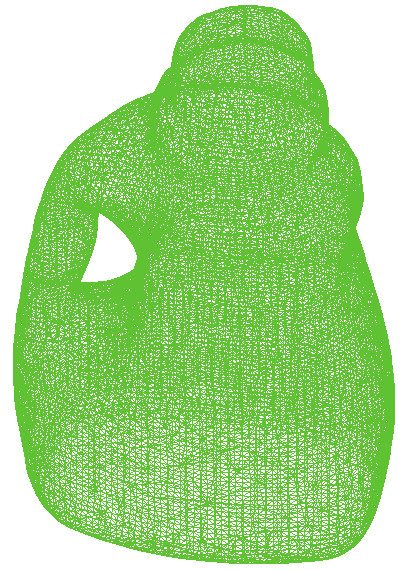
\includegraphics[width=\linewidth]{Figures/ObjRecog/mesh.png}
    \caption{Mesh}
    \label{fig:objrecog:meshcloudgrid:mesh}
  \end{subfigure}
  \begin{subfigure}{0.3\linewidth}
    \centering
    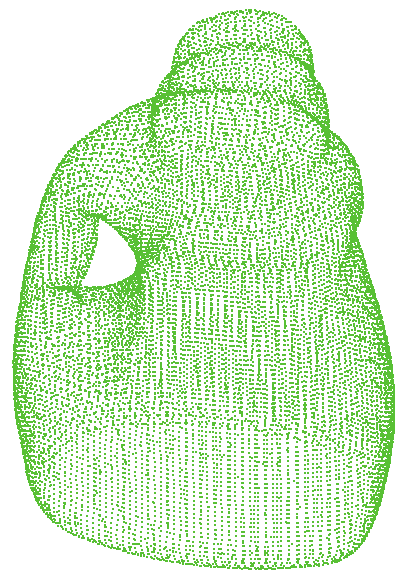
\includegraphics[width=\linewidth]{Figures/ObjRecog/cloud.png}
    \caption{Cloud}
    \label{fig:objrecog:meshcloudgrid:cloud}
  \end{subfigure}
  \begin{subfigure}{0.3\linewidth}
    \centering
    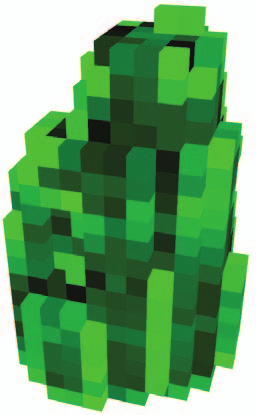
\includegraphics[width=0.9\linewidth]{Figures/ObjRecog/grid.png}
    \caption{Grid}
    \label{fig:objrecog:meshcloudgrid:grid}
  \end{subfigure}
  \caption{Various 3D representations for an object. A mesh (\subref{fig:objrecog:meshcloudgrid:mesh}) is transformed into a point cloud (\subref{fig:objrecog:meshcloudgrid:cloud}), and that cloud is processed to obtain a voxelized occupancy grid (\subref{fig:objrecog:meshcloudgrid:grid}). The occupancy grid shown in this figure is a cube of $30\times 30 \times 30$ voxels. Each voxel of that cube holds the point density inside its volume. In this case, dark voxels indicate high density whilst bright ones are low density volumes. Empty voxels were removed for better visualization.}
  \label{fig:objrecog:meshcloudgrid}
\end{figure}

With PointNet, we propose an occupancy grid inspired by the aforementioned successes but aiming to maintain a reasonable accuracy while allowing a real-time implementation. In our volumetric representation, each point of a cloud is mapped to a voxel of a fixed-size occupancy grid. Before performing that mapping, the object cloud is scaled to fit the grid. Each voxel will hold a value representing the number of points mapped to itself. At last, the values held by each cell are normalized. Figure \ref{fig:objrecog:meshcloudgrid} shows the derivation of the proposed occupancy grid representation from other typical tridimensional representations of a sample object.

\subsection{Network Architecture}
\label{cha:objrecog:sec:pointnet:subsec:network}

\begin{figure}[!t]
  \centering
  \includegraphics{example-image}
  \caption{PointNet's 3D \ac{CNN} architecture. [MISSINGDETAILS]}
  \label{fig:objrecog:pointnetarch}
\end{figure}

As we have previously stated, \acp{CNN} have proven to be very useful for recognizing and classifying objects in 2D images. A convolutional layer can recognize basic patterns such as corners or planes and if we stack several of them they can learn a topology of hierarchical filters that highlight regions of the images. What is more, the composition of several of these regions can define a feature of a more complex object. In this regard, a combination of various filters is able to recognize a full object. We apply this approach used in 2D images to 3D recognition. The deep architecture featured by PointNet is represented in Figure \ref{fig:objrecog:pointnetarch}. This setup allows PointNet to be on par with state-of-the-art algorithms while keeping reduced execution times.

\subsection{Experiments}
\label{cha:objrecog:sec:pointnet:subsec:experiments}

% TODO: Experiment details and procedure

\subsubsection{Data Generation}

\begin{figure}[!t]
  \centering
  \begin{subfigure}{\linewidth}
    \includegraphics[width=\linewidth, height=5cm]{example-image}
    \caption{Rendered views.}
    \label{fig:objrecog:dataproc:renders}
  \end{subfigure}
  \begin{subfigure}{0.32\linewidth}
    \includegraphics[width=\linewidth]{example-image}
    \caption{Mesh.}
    \label{fig:objrecog:dataproc:mesh}
  \end{subfigure}
  \begin{subfigure}{0.32\linewidth}
    \includegraphics[width=\linewidth]{example-image}
    \caption{Cloud.}
    \label{fig:objrecog:dataproc:cloud}
  \end{subfigure}
  \begin{subfigure}{0.32\linewidth}
    \includegraphics[width=\linewidth]{example-image}
    \caption{Downsampled.}
    \label{fig:objrecog:dataproc:downsampled}
  \end{subfigure}
  \caption{Dataset model processing example to generate the point clouds for PointNet. Some rendered views of a toilet model are shown in (\subref{fig:objrecog:dataproc:renders}). The original \ac{OFF} mesh is shown in (\subref{fig:objrecog:dataproc:mesh}). The generated point cloud after merging all points of view is shown in (\subref{fig:objrecog:dataproc:cloud}), and (\subref{fig:objrecog:dataproc:downsampled}) shows the downsampled cloud using a voxel grid filter with a leaf size of $0.7 \times 0.7 \times 0.7$.}
  \label{fig:objrecog:pointnetarch}
\end{figure}

The CAD models are provided in \ac{OFF}. Firstly, we converted all \ac{OFF} models into \ac{PLY} to ease the usage of the dataset with the \ac{PCL}. As we already mentioned, the input for PointNet are point clouds, but the dataset provides \ac{CAD} models specifying vertices and faces. In this regard, we converted the PLY models into \ac{PCD} clouds by raytracing them. A 3D sphere is tessellated and a virtual camera is placed in each vertex of that truncated icosahedron – pointing to the origin of the model – then multiple snapshots are rendered using raytracing and the z-buffer data, which contains the depth information, is used to generate point clouds from each point of view. After all points of view have been processed, the point clouds are merged. A voxel grid filter is applied to downsample the clouds after the raytracing operations. Figure 3 illustrates the aforementioned processes. After that, the resulting point clouds are used to train, randomizing the order of the models, and test the system taking into account the corresponding splits.

\subsubsection{Implementation}

This architecture was implemented using the \ac{PCL} \cite{Rusu2011}\cite{Aldoma2012} – which provides state-of-the-art algorithm implementations for 3D point cloud processing – and Caffe \cite{Jia2014}, a deep learning framework developed and maintained by the \ac{BVLC} and an active community of contributors on GitHub \footnote{\url{https://github.com/BVLC/caffe}}. This BSD-licensed C++ library enables researchers to design, train, and deploy \ac{CNN} architectures efficiently, mainly thanks to its drop-in integration of NVIDIA cuDNN \cite{Chetlur2014} to take advantage of \ac{GPU} acceleration.

% TODO: Source code

\subsubsection{Setup}

All the timings and results were obtained by performing the experiments in the following test setup: Intel Core i5-3570 with 8 GB of 1600 MHz DD3 RAM on an ASUS P8H77-M PRO motherboard (Intel H77 chipset). Additionally, the system includes an NVIDIA Tesla K20 GPU, and a Seagate Barracuda 7200.14 secondary storage. Caffe RC2 was run over ElementaryOS Freya 0.3.1, an Ubuntu-based Linux distribution. It was compiled using CMake 2.8.7, g++ 4.8.2, CUDA 7.0, and cuDNN v3.

\subsubsection{Results and Discussion}
\label{cha:objrecog:sec:pointnet:subsec:discussion}

As a result of training PointNet with a learning rate of 0.0001 and a momentum of 0.9 during 200 iterations using the ModelNet-10 dataset, it obtained a success rate of $77.6$\%. As shown in Figure 4, the confusion matrix reveals the stability of the system, mainly confusing items that look alike such as desk and table. Because of the nature of the \acp{CNN}, which heavily rely on detecting combinations of features, these kind of errors are common. As we can observe in Figure 5, the visual features that define a desk and a table are almost the same, making it hard to distinguish. Figure 6 shows the neuron activations for the output layer of the architecture, proving that Desk and Table are consistently confused during the tests. In light of these experiments, and taking into account the knowledge of the \acp{CNN} principles, it is conceivable to think that a deeper network would provide better results so more experiments were carried out.

In the deeper network experiment we added several layers to the PointNet architecture. One more convolutional layer was added since these layers are coupled to the detection of the features of the objects, so the more layers there are, a better or more expressive model is produced. An Inner Product layer was also added. Since these layers make the classification possible, adding more of them would theoretically provide better classification results.

This architecture was trained during $1,000$ iterations and tested every $200$ iterations. The best result was provided by the $800$ iterations test with an accuracy of $76.7$\%, while the $1,000$ iterations test dropped the performance to a $75.9$\% due to overfitting.

It is well known that training using an unbalanced dataset tends to harm those classes with the least number of examples and to benefit those with the most, as stated by [MISSINGREF]. Having this in mind, and knowing that ModelNet-10 is highly unbalanced as shown in Table [MISSINGTABLE], the dataset was balanced by limiting the number of examples of each class to $400$ using random undersampling. This does not fully solve the problem but improves the difference between the classes with the least number of examples and those with the most.

The network was trained and tested with this more balanced dataset using the architecture defined in Section III-B and it achieved an accuracy of $72.9$\%. The fact is that balancing the training set makes the accuracy of the classes with less examples higher, but it harms the success rate on classes with more, as seen in Figure [MISSINGREF].

After analyzing the results, it can be stated that neither a deeper network nor balancing the dataset increase accuracy. In fact, the experiments of the original architecture with the unbalanced ModelNet-10 offered the best recognition results with a $77.6$\% success rate. In addition, PointNet featuring the architecture exposed in Figure [MISSINGREF] takes an average time of $24.6$ miliseconds to classify an example (in comparison with Voxnet, which can take up to half a second for its raytracing-based implementation). These results prove the system as a fast and accurate 3D object class recognition tool.

\subsection{Conclusion}
\label{cha:objrecog:sec:pointnet:subsec:conclusion}

PointNet is a brand new kind of CNN for object class recognition that handles tridimensional data, inspired by VoxNet and 3D ShapeNets but using density occupancy grids as inner representation for input data. It was implemented in Caffe and provides a faster method than the state of art ones yet obtaining a high success rate as the experiments over the ModelNet10 dataset. This fact enlightens a promising future in real-time 3D recognition tasks.

Following on this work, we plan to improve the inner representation by using adaptable occupancy grids instead of fixed-size ones. In addition, we will integrate the system in an object recognition pipeline for 3D scenes. Our network will receive a point cloud segment of the scene where the object lies, produced by a preprocessing method, and that segments will be used to generate the occupancy grids that will be learned by the system. This implies adapting the system for learning partial views of the objects and dealing with occlusions and scale changes. As an additional feature, we will include pose estimation in that pipeline, all of this with goal of developing an end-to-end 3D object recognition system.

\section{Noise and Occlusion}
\label{cha:objrecog:sec:study}

\section{LonchaNet}
\label{cha:objrecog:sec:lonchanet}

\section{Conclusion}
\label{cha:objrecog:sec:conclusion}
